\documentclass{templateNote}
\usepackage{tcolorbox}
\usepackage{pgfplots}
\usepackage{amsmath}

\begin{document}

\imagenlogoU{img/LogoElNube.png}
\linklogoU{https://github.com/MarceloPazPezo}
\linkDoc{https://github.com/MarceloPazPezo/MyRepo/blob/main/Icinf/Semestre\%203/Calculo\%20Integral/Suma\%20de\%20Riemann/Suma\%20De\%20Riemann.pdf}
\universidad{Universidad del Bío-Bío}
\titulo{Suma de Riemann} % Titulo
\asignatura{Calculo Integral} % Asignatura
\autor{
    \indent
    Marcelo \textsc{Paz}
}   
\portada
\margenes % Crear márgenes


\section{Teoria}
\subsection{Algunas Sumatorias}

\[
    \sum_{i=0}^{n}1=n \quad \quad \sum_{i=1}^{n}C = C\sum_{i=1}^{n}1=Cn \quad \quad \sum_{i=1}^{n}i = \frac{n(n+1)}{2}
\]
\\
\[
    \sum_{i=1}^{n}i^2 = \frac{n(n+1)(2n+1)}{6} \quad \quad \sum_{i=1}^{n}i^3 = \left( \frac{n(n+1)}{2} \right)^2
\]
\\
\[
    \sum_{i=1}^{n}(i^2 + i -2) = \sum_{i=1}^{n}i^2 + \sum_{i=1}^{n}i - \sum_{i=1}^{n}2 = \frac{n(n+1)(2n+1)}{6} + \frac{n(n+1)}{2} - 2n
\]

\subsection{Suma de Riemann}
\indent
Método de aproximar el área bajo un gráfico al sumar un número entero de áreas rectangulares dibujadas bajo la curva.

\[
    \sum_{i=1}^{n}f(x_i)\,\Delta x \quad \text{, donde} \quad \Delta x = \frac{b-a}{n} \text{ , } \quad n = \text{ número de subdivisiones, } \quad x_i \in \text{[} a, b\text{]}
\]

\begin{figure}[H]
    \centering
    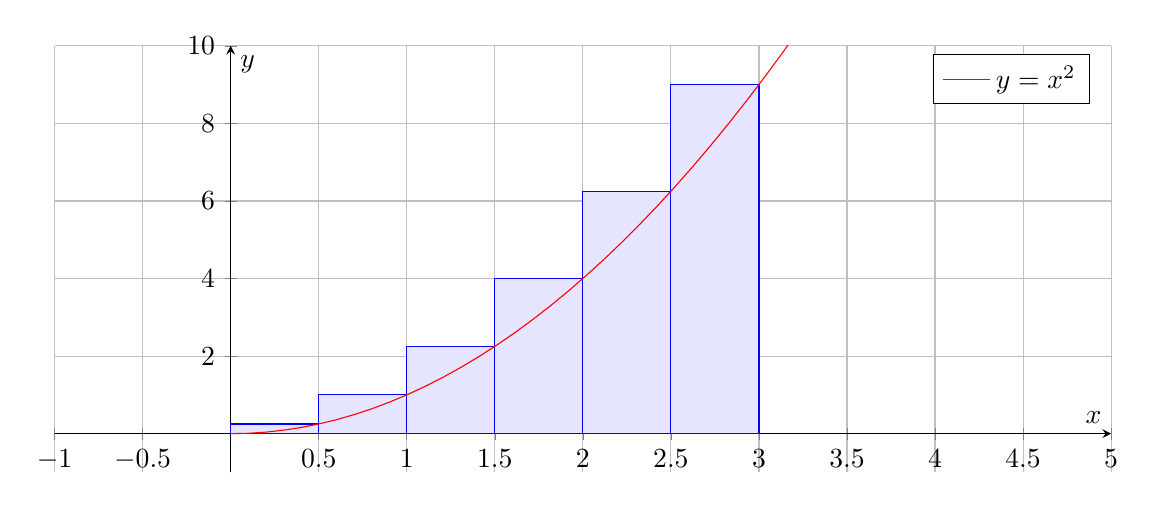
\begin{tikzpicture}[scale=1]
        \begin{axis}[
            axis lines = middle,
            xlabel = \(x\),
            ylabel = \(y\),
            ymin = -1,
            ymax = 10,
            xmin = -1,
            xmax = 5,
            grid = major,
            width = 15cm,
            height = 7cm,
        ]
        \draw [blue, fill=blue!10] (axis cs:0,0) rectangle (axis cs:{1/2},{(1/2)^2});
        \draw [blue, fill=blue!10] (axis cs:1/2,0) rectangle (axis cs:{2/2},{(2/2)^2});
        \draw [blue, fill=blue!10] (axis cs:2/2,0) rectangle (axis cs:{3/2},{(3/2)^2});
        \draw [blue, fill=blue!10] (axis cs:3/2,0) rectangle (axis cs:{4/2},{(4/2)^2});
        \draw [blue, fill=blue!10] (axis cs:4/2,0) rectangle (axis cs:{5/2},{(5/2)^2});
        \draw [blue, fill=blue!10] (axis cs:5/2,0) rectangle (axis cs:{6/2},{(6/2)^2});
        \addplot [
            domain=0:10, 
            samples=100, 
            color=red,
        ]
        {x^2};
        \addlegendentry{\(y=x^2\)}
        \end{axis}
    \end{tikzpicture}
    \caption{Suma de Riemann}
\end{figure}

\newpage
\subsection{Suma izquierda de Riemann}
\indent
El $x_i$ de cada rectángulo es el extremo izquierdo, $m_i = a+(i-1)(\frac{b-a}{n})$.

\[
    \sum_{i=1}^{n}f(m_i)\,\Delta x \quad \text{, donde} \quad \Delta x = \frac{b-a}{n} \text{ , } \quad n = \text{ número de subdivisiones, } \quad m_i \in \text{[} a, b- \Delta x \text{]}
\]

\begin{figure}[H]
    \centering
    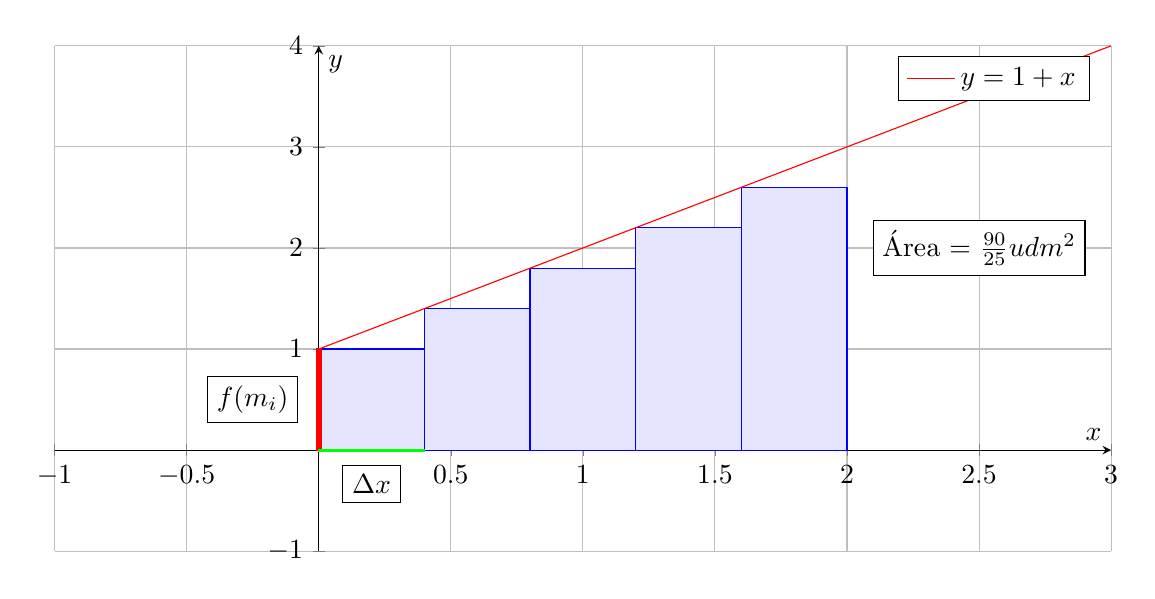
\begin{tikzpicture}[scale=1]
        \begin{axis}[
            axis lines = middle,
            xlabel = \(x\),
            ylabel = \(y\),
            ymin = -1,
            ymax = 4,
            xmin = -1,
            xmax = 3,
            grid = major,
            width = 15cm,
            height = 8cm,
        ]
        \draw [blue, fill=blue!10] (axis cs:0,0) rectangle (axis cs:{2/5},{1});
        \draw [blue, fill=blue!10] (axis cs:{2/5},0) rectangle (axis cs:{4/5},{1+2/5});
        \draw [blue, fill=blue!10] (axis cs:{4/5},0) rectangle (axis cs:{6/5},{1+4/5});
        \draw [blue, fill=blue!10] (axis cs:{6/5},0) rectangle (axis cs:{8/5},{1+6/5});
        \draw [blue, fill=blue!10] (axis cs:{8/5},0) rectangle (axis cs:{10/5},{1+8/5});
        \draw [red, fill=red!100] (axis cs:-0.01,0) rectangle (axis cs:0.01,{1});
        \draw [green, fill=green!100] (axis cs:0,-0.01,) rectangle (axis cs:{2/5},0.01);
        \addplot [
            domain=0:5, 
            samples=100, 
            color=red,
        ]
        {1+x};
        \addlegendentry{\(y=1+x\)}
        \node[draw, fill=white] at (axis cs:5/2,2) {Área = $\frac{90}{25} udm^2$};
        \node[draw, fill=white] at (axis cs:{1/5},{-1/3}) {$\Delta x$};
        \node[draw, fill=white] at (axis cs:{-3/12},{2/4}) {$f(m_i)$};
        \end{axis}
    \end{tikzpicture}
    \caption{Suma izquierda de Riemann}
\end{figure}

\subsection{Suma derecha de Riemann}
\indent
El $x_i$ de cada rectángulo es el extremo derecho, $M_i = a+i(\frac{b-a}{n})$.
\[
    \sum_{i=1}^{n}f(M_i)\,\Delta x \quad \text{, donde} \quad \Delta x = \frac{b-a}{n} \text{ , } \quad n = \text{ número de subdivisiones, } \quad M_i \in \text{[} a+\Delta x, b\text{]}
\]

\begin{figure}[H]
    \centering
    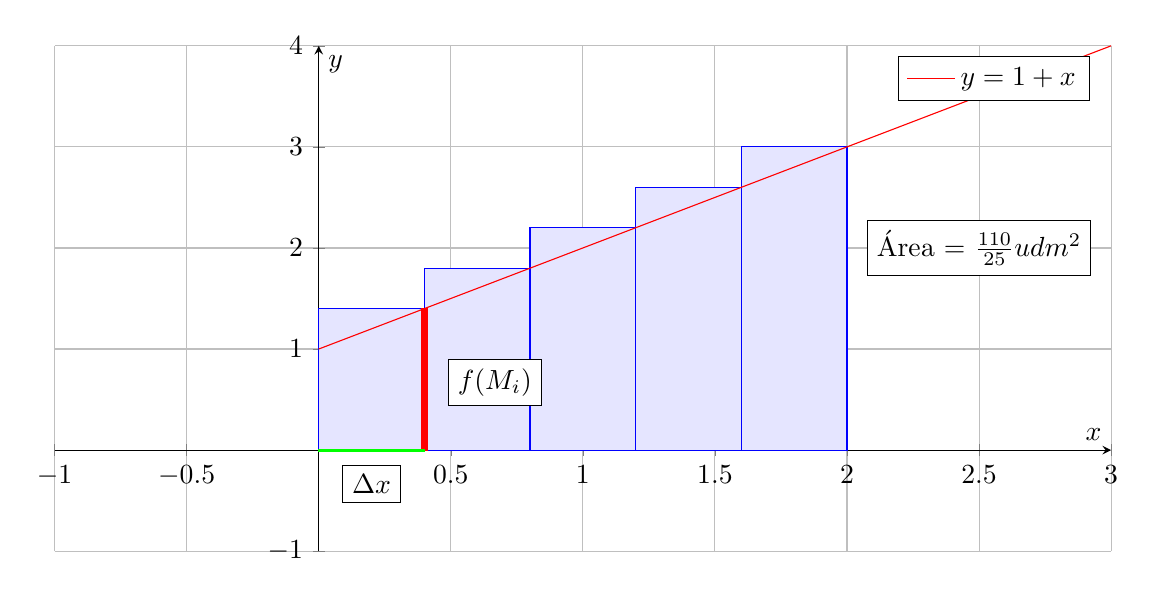
\begin{tikzpicture}[scale=1]
        \begin{axis}[
            axis lines = middle,
            xlabel = \(x\),
            ylabel = \(y\),
            ymin = -1,
            ymax = 4,
            xmin = -1,
            xmax = 3,
            grid = major,
            width = 15cm,
            height = 8cm,
            ]
        \draw [blue, fill=blue!10] (axis cs:0,0) rectangle (axis cs:{2/5},{1+2/5});
        \draw [blue, fill=blue!10] (axis cs:{2/5},0) rectangle (axis cs:{4/5},{1+4/5});
        \draw [blue, fill=blue!10] (axis cs:{4/5},0) rectangle (axis cs:{6/5},{1+6/5});
        \draw [blue, fill=blue!10] (axis cs:{6/5},0) rectangle (axis cs:{8/5},{1+8/5});
        \draw [blue, fill=blue!10] (axis cs:{8/5},0) rectangle (axis cs:{10/5},{1+10/5});
        \draw [red, fill=red!100] (axis cs:{2/5 - 0.01},0) rectangle (axis cs:{2/5 + 0.01},{1+2/5});
        \draw [green, fill=green!100] (axis cs:0,-0.01,) rectangle (axis cs:{2/5},0.01);
        \addplot [
            domain=0:5, 
            samples=100, 
            color=red,
        ]
        {1+x};
        \addlegendentry{\(y=1+x\)}
        \node[draw, fill=white] at (axis cs:5/2,2) {Área = $\frac{110}{25} udm^2$};
        \node[draw, fill=white] at (axis cs:{1/5},{-1/3}) {$\Delta x$};
        \node[draw, fill=white] at (axis cs:{8/12},{2/3}) {$f(M_i)$};
        \end{axis}
    \end{tikzpicture}
    \caption{Suma derecha de Riemann}
\end{figure}

\newpage
\section{Ejercicios}
\subsection{Ejercicio 1}
\indent
Determinar aproximadamente el area bajo la curva $y = f(x) = 1+x$ entre $x=0$ y $x=2$, dividiendo el intervalo $[a,b]$ en 5 subintervalos de igual longitud. Realice dos aproximaciones, la primera usando el lado izquierdo de cada subintervalo y la segunda usando su lado derecho.

\subsubsection{Datos}
\[
    n = 5 \quad \quad a = 0 \quad \quad b = 2 \quad \quad f(x) = 1+x
\]
\\
\begin{align*}
    \text{Area Exacta} &= \int_{0}^{2} (1+x) dx \\
    &= \left. x + \frac{x^2}{2} \right|_{0}^{2} \\
    &= 2 + \frac{4}{2} - \left( 0 + \frac{0^2}{2}\right) \\
    &= 4 udm^2
\end{align*}

\begin{figure}[H]
    \centering
    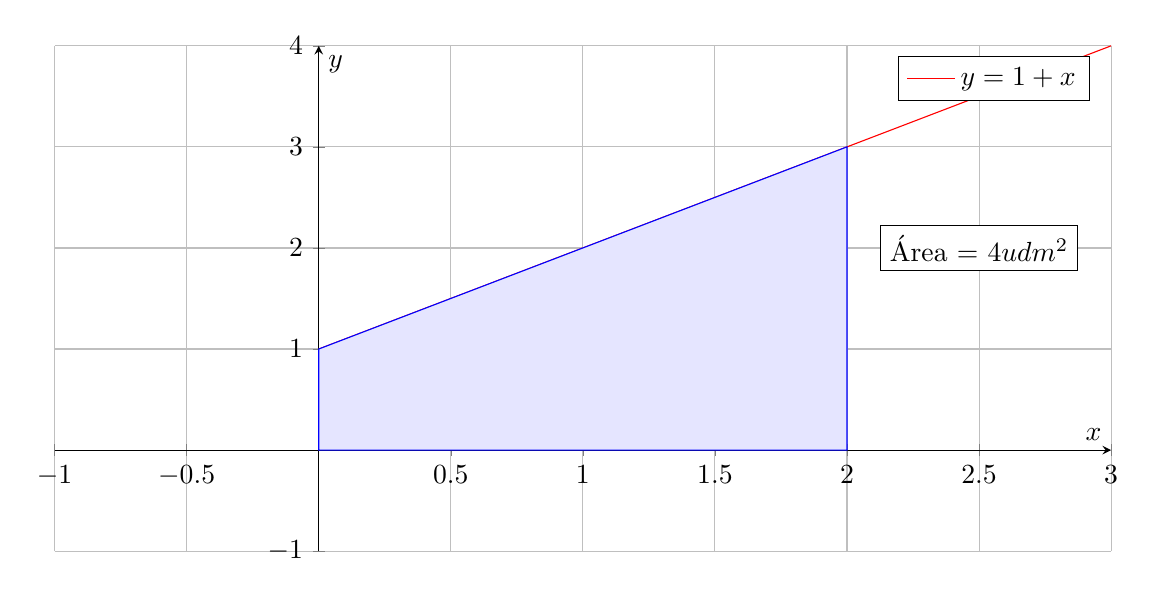
\begin{tikzpicture}[scale=1]
        \begin{axis}[
            axis lines = middle,
            xlabel = \(x\),
            ylabel = \(y\),
            ymin = -1,
            ymax = 4,
            xmin = -1,
            xmax = 3,
            grid = major,
            width = 15cm,
            height = 8cm,
        ]
        \addplot [
            domain=0:5, 
            samples=100, 
            color=red,
        ]
        {1+x};
        \addlegendentry{\(y=1+x\)}
        \node[draw, fill=white] at (axis cs:5/2,2) {Área = $4 udm^2$};
        \draw [blue, fill=blue!10] (axis cs:0,0) -- (axis cs:2,0) -- (axis cs:2,3) -- (axis cs:0,1) -- cycle;
    
        \end{axis}
    \end{tikzpicture}
    \caption{Integral desde 0 a 2 de $f(x)=1+x$}
\end{figure}

\newpage
\subsubsection{Suma izquierda}
\[
    m_i = 0 + (i-1) \left( \frac{2-0}{5} \right) = \frac{2}{5}(i-1)
\]

\begin{align*}
    s(5) &= \sum_{i=1}^{5}f\left(\frac{2}{5}(i-1)\right)\frac{2}{5} && \text{Remplazamos los datos en la ecuación} \\
    &= \sum_{i=1}^{5} \left(1+\frac{2}{5}(i-1)\right)\frac{2}{5} && \text{Evaluamos en la función} \\
    &= \frac{2}{5} \sum_{i=1}^{5} \left( \frac{2}{5}(i-1) + 1 \right) && \text{Sacamos la constante $\frac{2}{5}$ de la sumatoria} \\
    &= \frac{2}{5} \left( \frac{2}{5} \sum_{i=1}^{5}(i-1) + \sum_{i=1}^{5}1\right) && \text{Separamos la sumatoria} \\
    &= \frac{2}{5} \left( \frac{2}{5} \left(\sum_{i=1}^{5}i - \sum_{i=1}^{5}1\right) + \sum_{i=1}^{5}1\right) && \text{Separamos la sumatoria} \\
    &= \frac{2}{5} \left( \frac{2}{5} \left(\frac{5 \times 6}{2} - 5\right) + 5\right) && \text{Resolvemos las sumatorias} \\
    &= \frac{2}{5} \left( \frac{2}{5} \times 10 + 5\right) \\
    &= \frac{2}{5} \left( 4 + 5\right) \\
    &= \frac{18}{5} \\
    &= \frac{90}{25} = 3,6udm^2\\
\end{align*}

\begin{figure}[H]
    \centering
    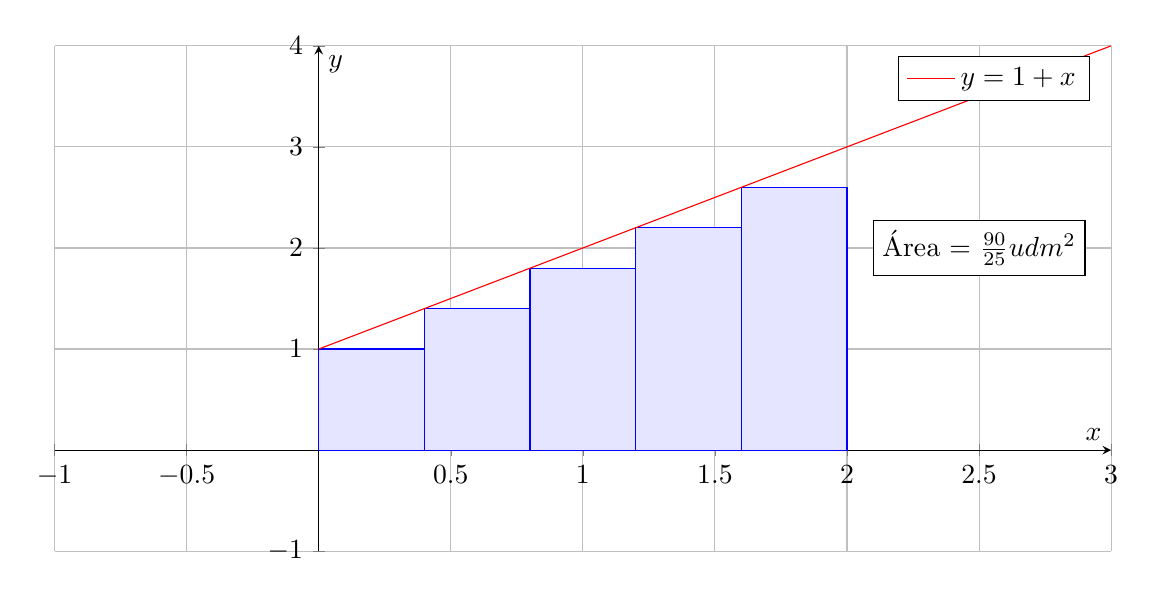
\begin{tikzpicture}[scale=1]
        \begin{axis}[
            axis lines = middle,
            xlabel = \(x\),
            ylabel = \(y\),
            ymin = -1,
            ymax = 4,
            xmin = -1,
            xmax = 3,
            grid = major,
            width = 15cm,
            height = 8cm,
        ]
        \draw [blue, fill=blue!10] (axis cs:0,0) rectangle (axis cs:{2/5},{1});
        \draw [blue, fill=blue!10] (axis cs:{2/5},0) rectangle (axis cs:{4/5},{1+2/5});
        \draw [blue, fill=blue!10] (axis cs:{4/5},0) rectangle (axis cs:{6/5},{1+4/5});
        \draw [blue, fill=blue!10] (axis cs:{6/5},0) rectangle (axis cs:{8/5},{1+6/5});
        \draw [blue, fill=blue!10] (axis cs:{8/5},0) rectangle (axis cs:{10/5},{1+8/5});
        \addplot [
            domain=0:5, 
            samples=100, 
            color=red,
        ]
        {1+x};
        \addlegendentry{\(y=1+x\)}
        \node[draw, fill=white] at (axis cs:5/2,2) {Área = $\frac{90}{25} udm^2$};

        \end{axis}
    \end{tikzpicture}
    \caption{Suma izquierda de Riemann}
\end{figure}

\newpage
\subsubsection{Suma derecha}
\[
    M_i = 0 + (i) \left( \frac{2-0}{5} \right) = \frac{2 i}{5}
\]

\begin{align*}
    s(5) &= \sum_{i=1}^{5}f\left(\frac{2 i}{5}\right)\frac{2}{5} && \text{Remplazamos los datos en la ecuación} \\
    &= \sum_{i=1}^{5} \left(1+\frac{2 i}{5}\right)\frac{2}{5} && \text{Evaluamos en la función} \\
    &= \frac{2}{5} \sum_{i=1}^{5} \left( \frac{2 i}{5} + 1 \right) && \text{Sacamos la constante $\frac{2}{5}$ de la sumatoria} \\
    &= \frac{2}{5} \left( \frac{2}{5} \sum_{i=1}^{5}i + \sum_{i=1}^{5}1\right) && \text{Separamos la sumatoria} \\
    &= \frac{2}{5} \left( \frac{2}{5} \left(\frac{5 \times 6}{2}\right) + 5\right) && \text{Resolvemos las sumatorias} \\
    &= \frac{2}{5} \left( 6 + 5\right) \\
    &= \frac{22}{5} \\
    &= \frac{110}{25} = 4,4 udm^2\\
\end{align*}

\begin{figure}[H]
    \centering
    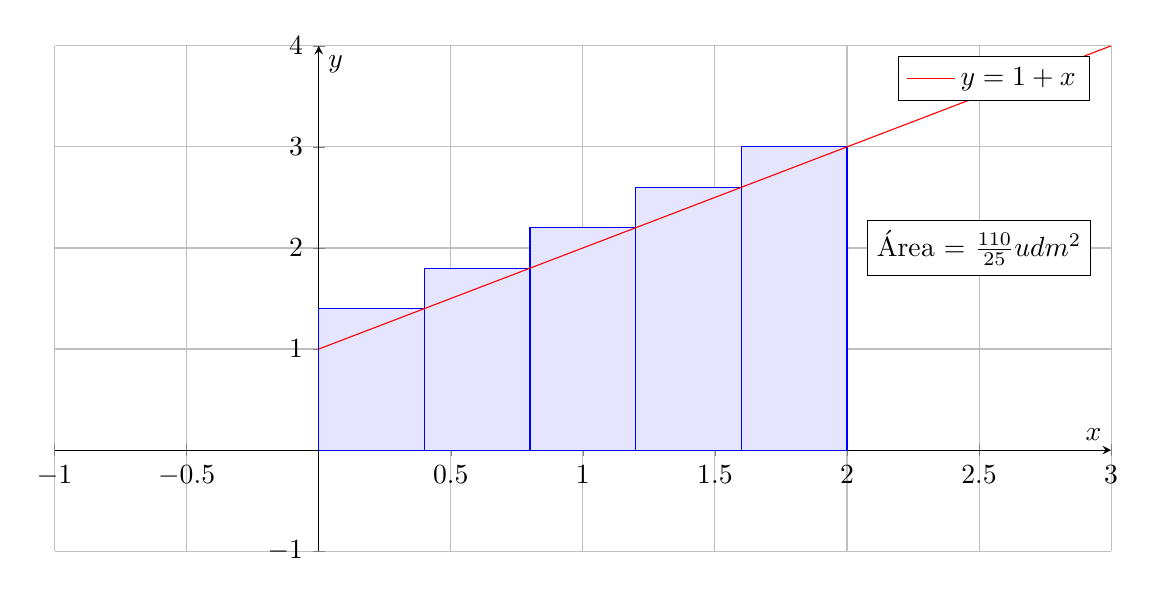
\begin{tikzpicture}[scale=1]
        \begin{axis}[
            axis lines = middle,
            xlabel = \(x\),
            ylabel = \(y\),
            ymin = -1,
            ymax = 4,
            xmin = -1,
            xmax = 3,
            grid = major,
            width = 15cm,
            height = 8cm,
        ]
        \draw [blue, fill=blue!10] (axis cs:0,0) rectangle (axis cs:{2/5},{1+2/5});
        \draw [blue, fill=blue!10] (axis cs:{2/5},0) rectangle (axis cs:{4/5},{1+4/5});
        \draw [blue, fill=blue!10] (axis cs:{4/5},0) rectangle (axis cs:{6/5},{1+6/5});
        \draw [blue, fill=blue!10] (axis cs:{6/5},0) rectangle (axis cs:{8/5},{1+8/5});
        \draw [blue, fill=blue!10] (axis cs:{8/5},0) rectangle (axis cs:{10/5},{1+10/5});
        \addplot [
            domain=0:5, 
            samples=100, 
            color=red,
        ]
        {1+x};
        \addlegendentry{\(y=1+x\)}
        \node[draw, fill=white] at (axis cs:5/2,2) {Área = $\frac{110}{25} udm^2$};
        \end{axis}
    \end{tikzpicture}
    \caption{Suma derecha de Riemann}
\end{figure}

\end{document}
